
\documentclass[11pt]{article}


% Use wide margins, but not quite so wide as fullpage.sty
\marginparwidth 0.2in 
\oddsidemargin 0.1in 
\evensidemargin 0.1in 
\marginparsep 0.1in
\topmargin 0.1in 
\textwidth 6.5in \textheight 8 in
% That's about enough definitions

% multirow allows you to combine rows in columns
\usepackage{multirow}
% tabularx allows manual tweaking of column width
\usepackage{tabularx}
% longtable does better format for tables that span pages
\usepackage{longtable}
\usepackage{graphicx}
\usepackage{amssymb} % needed for math
\usepackage{amsmath} % needed for math
\usepackage{listings} % needed for the inclusion of source code       
\usepackage{mips}

\usepackage{color}

\definecolor{dkgreen}{rgb}{0,0.6,0}
\definecolor{gray}{rgb}{0.5,0.5,0.5}
\definecolor{mauve}{rgb}{0.58,0,0.82}

\lstset{ %
  language=[mips]Assembler,       % the language of the code
  basicstyle=\footnotesize,       % the size of the fonts that are used for the code
  numbers=left,                   % where to put the line-numbers
  numberstyle=\tiny\color{gray},  % the style that is used for the line-numbers
  stepnumber=1,                   % the step between two line-numbers. If it's 1, each line 
                                  % will be numbered
  numbersep=5pt,                  % how far the line-numbers are from the code
  backgroundcolor=\color{white},  % choose the background color. You must add \usepackage{color}
  showspaces=false,               % show spaces adding particular underscores
  showstringspaces=false,         % underline spaces within strings
  showtabs=false,                 % show tabs within strings adding particular underscores
  frame=single,                   % adds a frame around the code
  rulecolor=\color{black},        % if not set, the frame-color may be changed on line-breaks within not-black text (e.g. commens (green here))
  tabsize=4,                      % sets default tabsize to 2 spaces
  captionpos=b,                   % sets the caption-position to bottom
  breaklines=true,                % sets automatic line breaking
  breakatwhitespace=false,        % sets if automatic breaks should only happen at whitespace
  title=\lstname,                 % show the filename of files included with \lstinputlisting;
                                  % also try caption instead of title
  keywordstyle=\color{blue},          % keyword style
  commentstyle=\color{dkgreen},       % comment style
  stringstyle=\color{mauve},         % string literal style
  escapeinside={\%*}{*)},            % if you want to add a comment within your code
  morekeywords={*,...}               % if you want to add more keywords to the set
}

\usepackage{hyperref}  

\begin{document}


\author{İbrahim Burak Tanrıkulu, 21827852}
\title{BBM436: Microprocessors Lab.\\2020-2021 Autumn\\Homework 2}
\maketitle

\section{Phase: Creating workspace}

\begin{itemize}
    \item {Firstly i used minecraft to create an 74181 ALU and i did half of it. But doing it in minecraft was time consuming. So i decided to use Proteus.}
    \item {I downloaded and installed Proteus and will use it.}
\end{itemize}

\section{Phase: Running Examples}

\begin{itemize}
    \item {I ran examples and did my first 74181 ALU in Proteus \ref{fig:74181} . I checked this ALU with random inputs.}
\end{itemize}

\section{Phase: Designing ALU and Register}

\begin{itemize}
    \item {I decided to do 16 bit ALU and Registers for to use in next projects.}
    \item {I designed 16-bit ALU with 74181 ALU \ref{fig:ALU} and 74182 Lookahead Carry Generator \ref{fig:Carry} . }
    \newline There are 4 piece of 74181 to make 16 bit ALU. Lookahead Carry Generator makes this ALUs faster.
    \item {I designed 16-bit register file with open-collector D Flip-Flops \ref{fig:REG} . }
    \newline Every register is 16 bit length and there are 16 registers in this register file. 
    \newline I used 16 piece of OR gate to multiplex these register BUSes.
    \item {I checked these circuits with pattern generator \ref{fig:Pattern} and logic analyzer \ref{fig:Analyze} . }
\end{itemize}
 
\newpage

\section{Phase: Sample 8086 compiler}

\begin{itemize}
	\item {I used emu8086 application to simulate 8086 microprocessor. Also i installed MASM32 .}
	\item {There is a sample addition/substraction code and simulation of this code. \ref{fig:emu8086} }
	\newline You can run it step by step or completely. While you stepping this commands, You can see assembly codes.
\end{itemize}

\section{Phase: Machine Code Extraction}

\begin{itemize}
	\item {I used another addition code to extract machine code. I will use WinHex to view these machine codes. }
	\newline sample.asm \ref{fig:WinHexAsm}
	\newline sample.obj \ref{fig:WinHexObj}
	\newline sample.exe \ref{fig:WinHexExe}
\end{itemize}

I can share my Proteus project and Minecraft map.

\begin{figure}[h!]
        \centering
        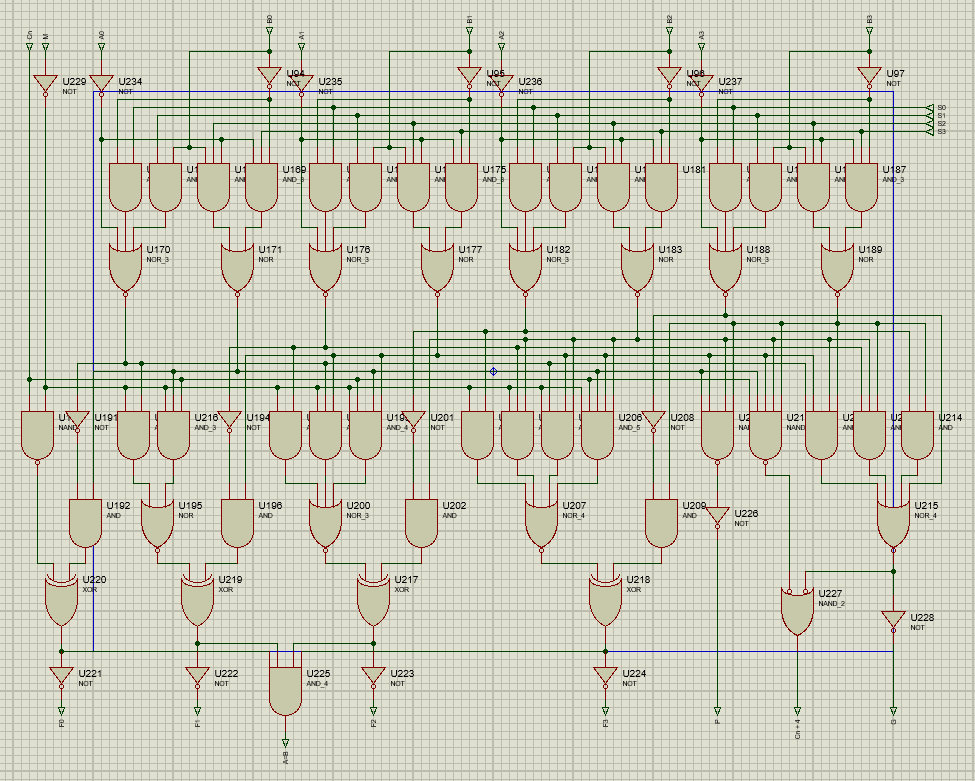
\includegraphics[width=17cm]{74181.png}
        \caption{74181 ALU}
        \label{fig:74181}
\end{figure}

\begin{figure}[h!]
        \centering
        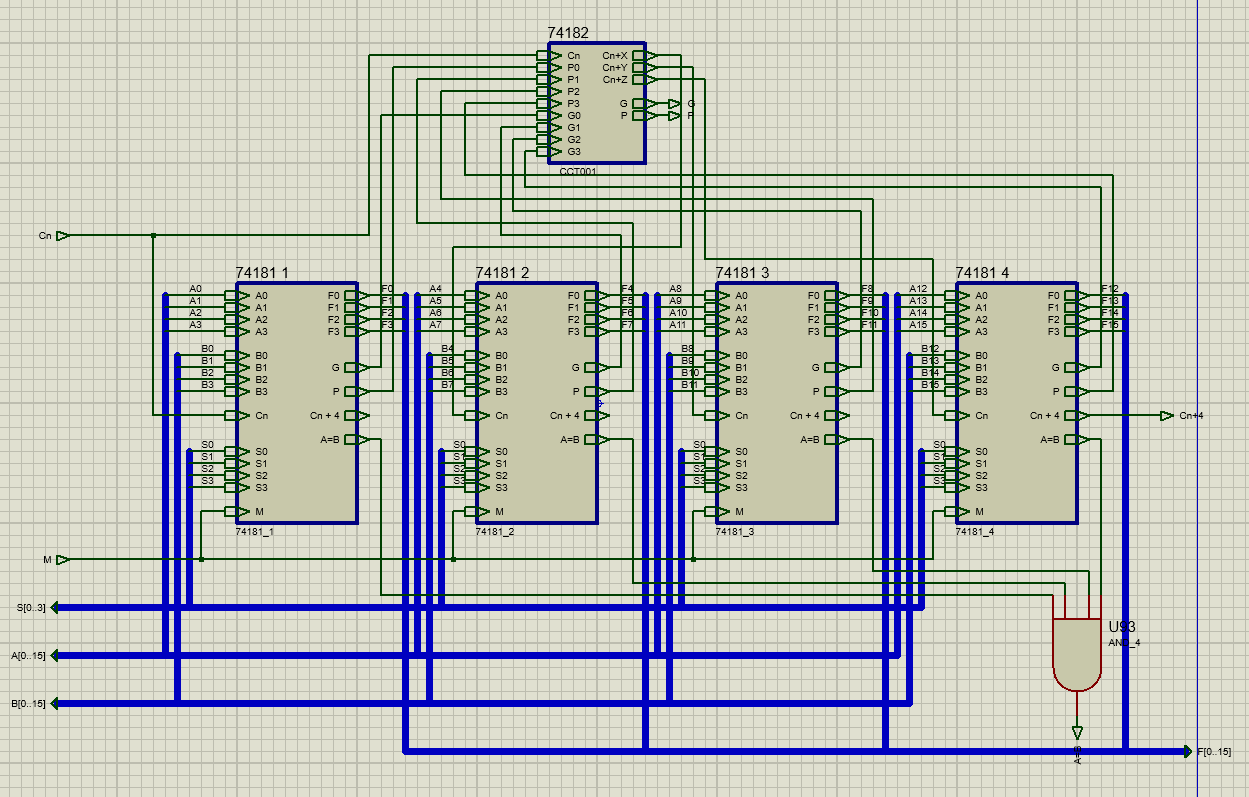
\includegraphics[width=17cm]{ALU.png}
        \caption{16-bit ALU}
        \label{fig:ALU}
\end{figure}

\begin{figure}[h!]
	\centering
	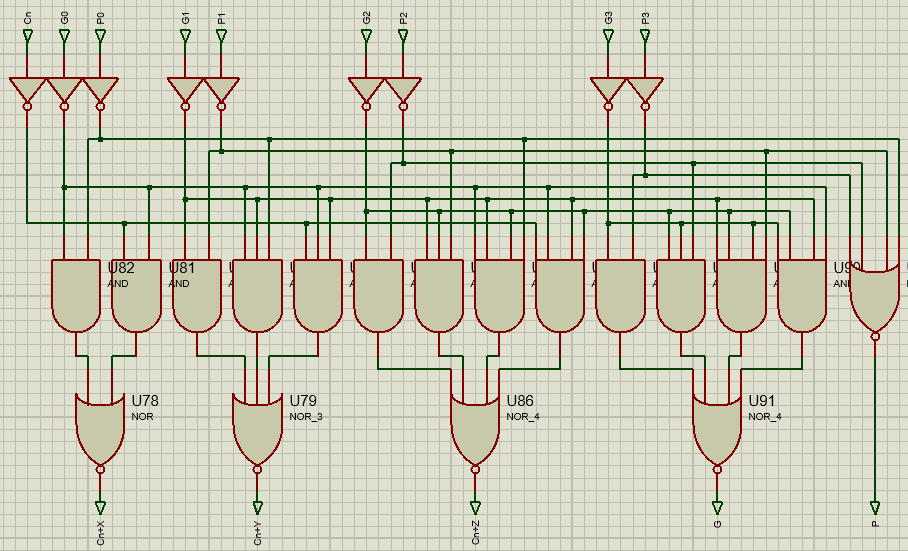
\includegraphics[width=13cm]{74182.png}
	\caption{74182 Lookahead Carry Generator}
	\label{fig:Carry}
\end{figure}

\begin{figure}[h!]
        \centering
        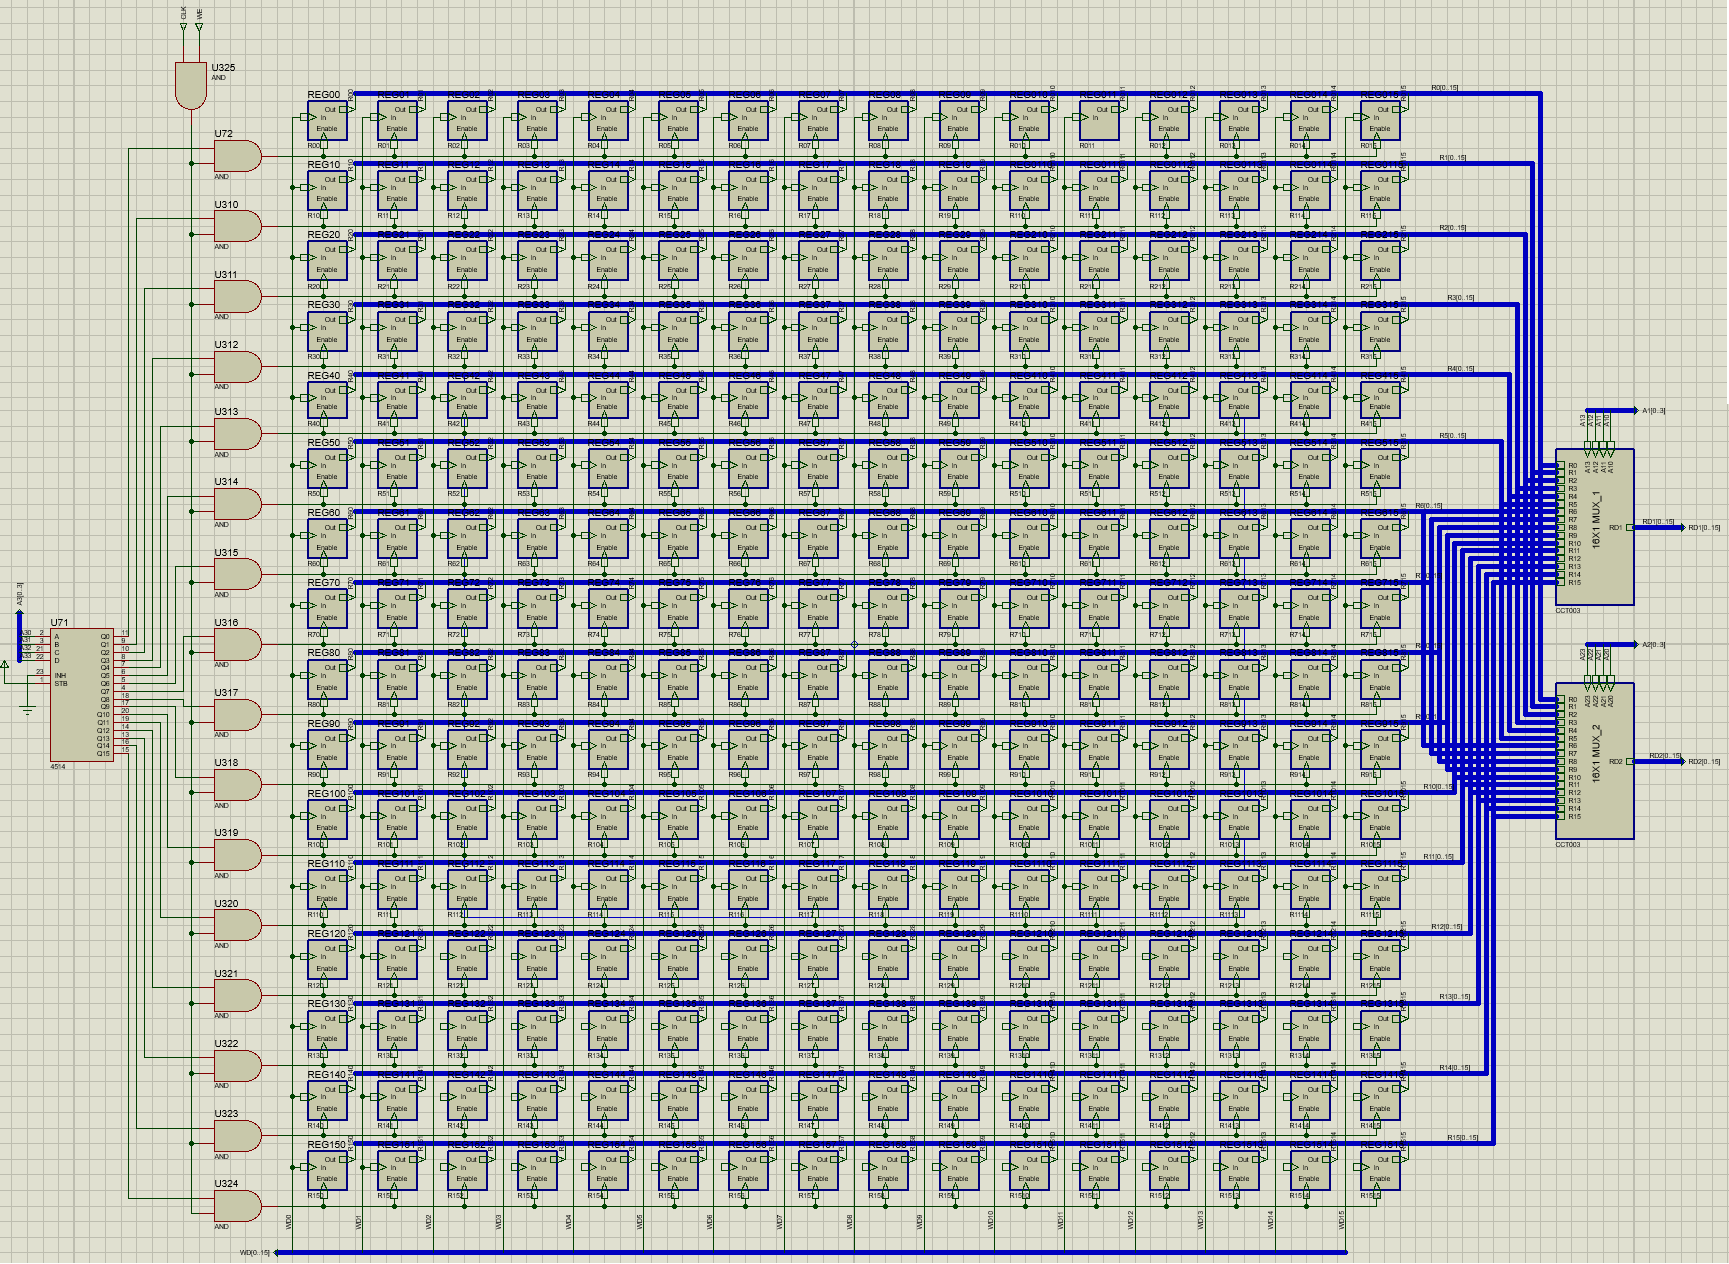
\includegraphics[width=17cm]{RegFile.png}
        \caption{16-bit Register File}
        \label{fig:REG}
\end{figure}

\begin{figure}[h!]
        \centering
        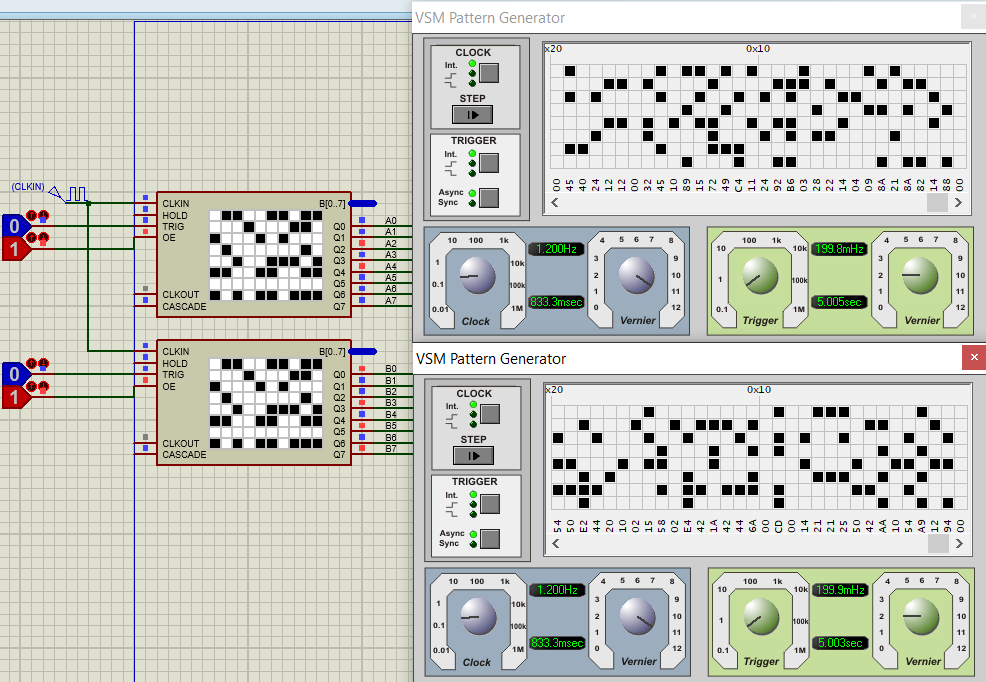
\includegraphics[width=12cm]{Pattern.png}
        \caption{Pattern Generator}
        \label{fig:Pattern}
\end{figure}

\begin{figure}[h!]
        \centering
        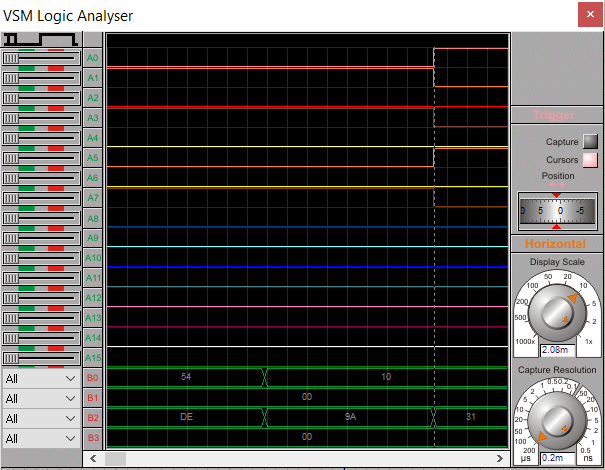
\includegraphics[width=12cm]{Analyze.png}
        \caption{Logic Analyzer}
        \label{fig:Analyze}
\end{figure}

\begin{figure}[h!]
        \centering
        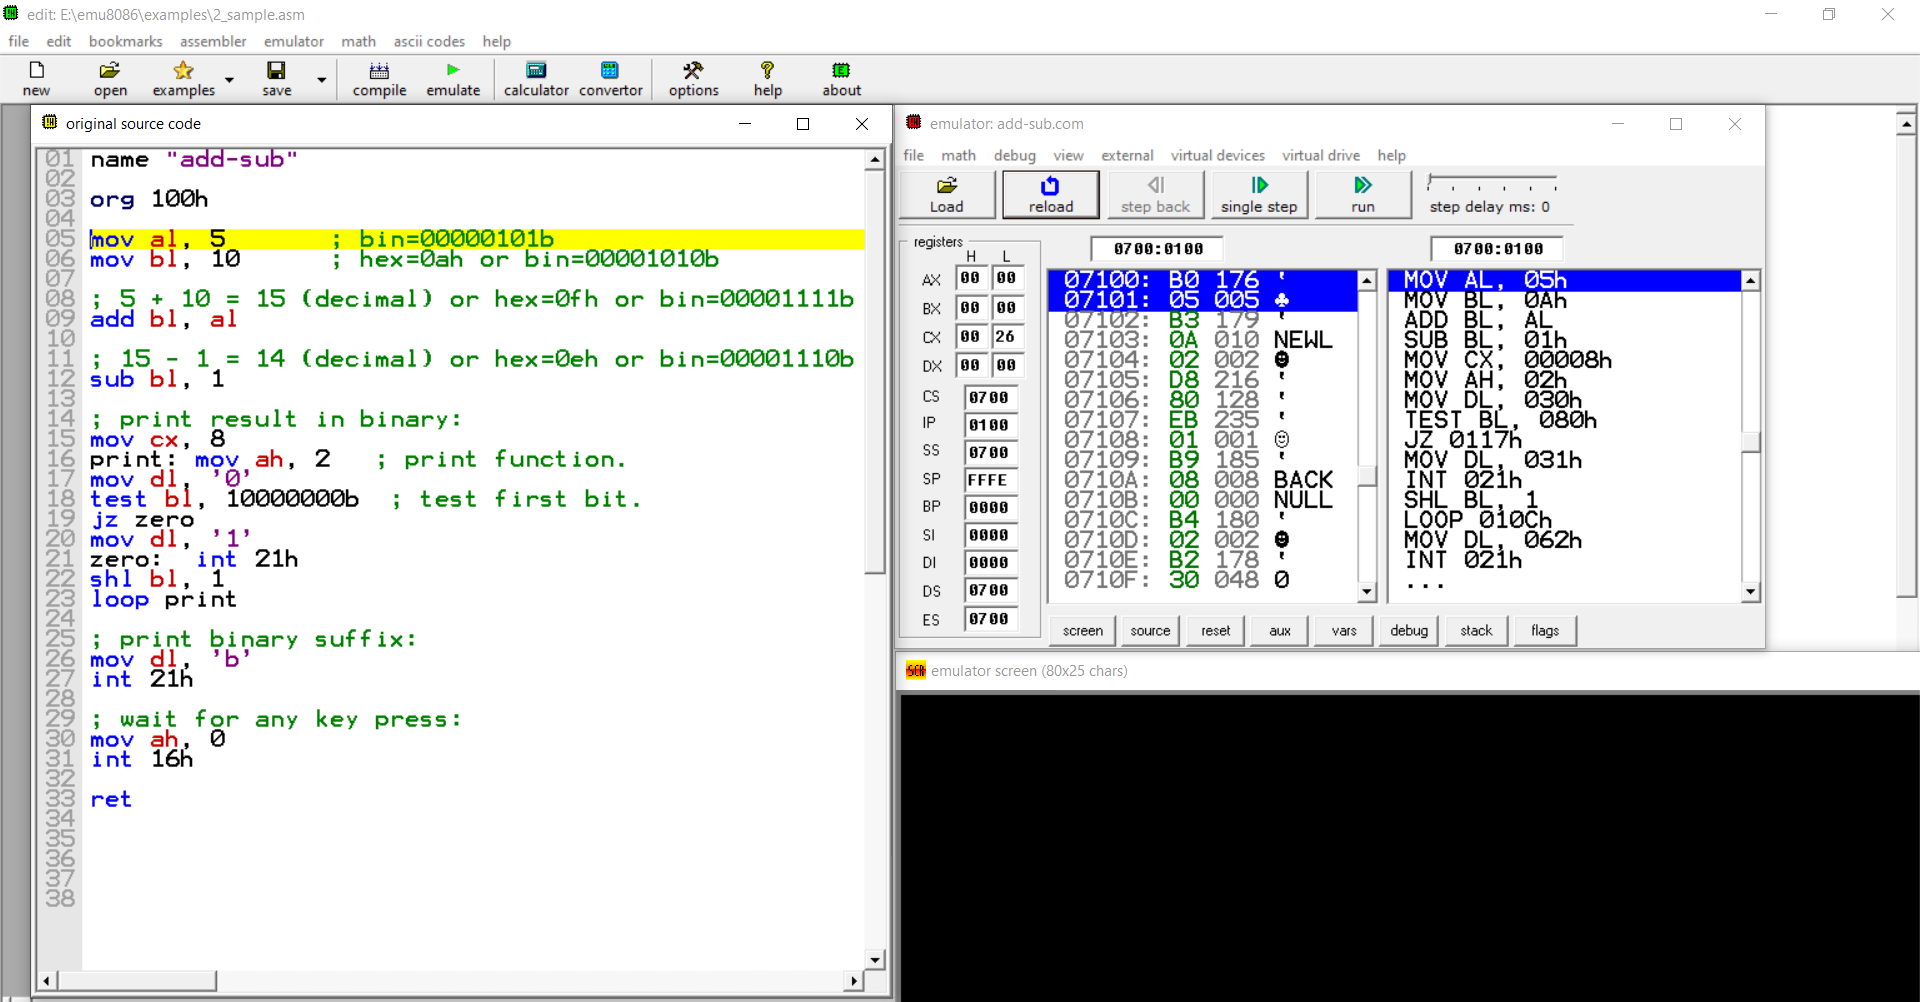
\includegraphics[width=17cm]{emu8086.png}
        \caption{Sample Program in emu8086}
        \label{fig:emu8086}
\end{figure}

\begin{figure}[h!]
        \centering
        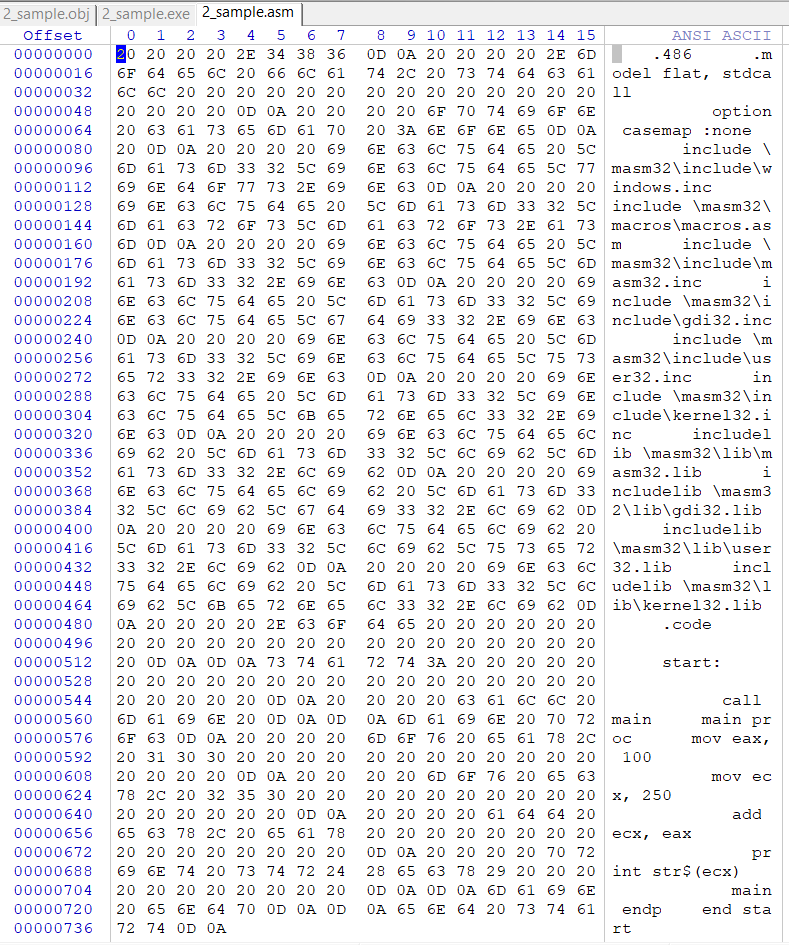
\includegraphics[width=17cm]{WinHexAsm.png}
        \caption{Assembly Code with WinHex}
        \label{fig:WinHexAsm}
\end{figure}

\begin{figure}[h!]
        \centering
        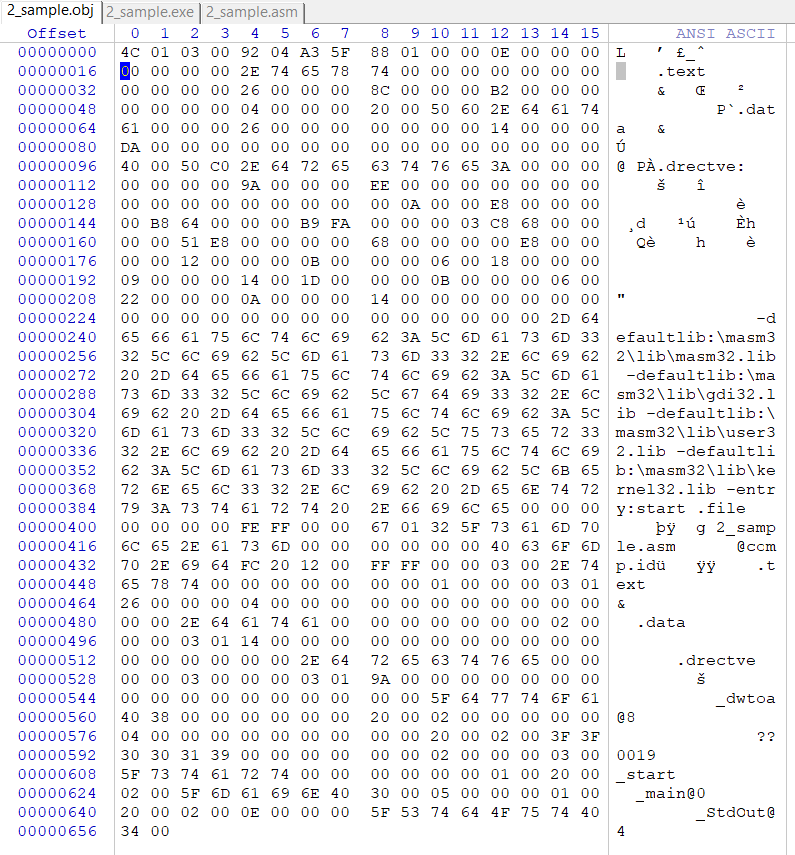
\includegraphics[width=17cm]{WinHexObj.png}
        \caption{Object Code with WinHex}
        \label{fig:WinHexObj}
\end{figure}

\begin{figure}[h!]
        \centering
        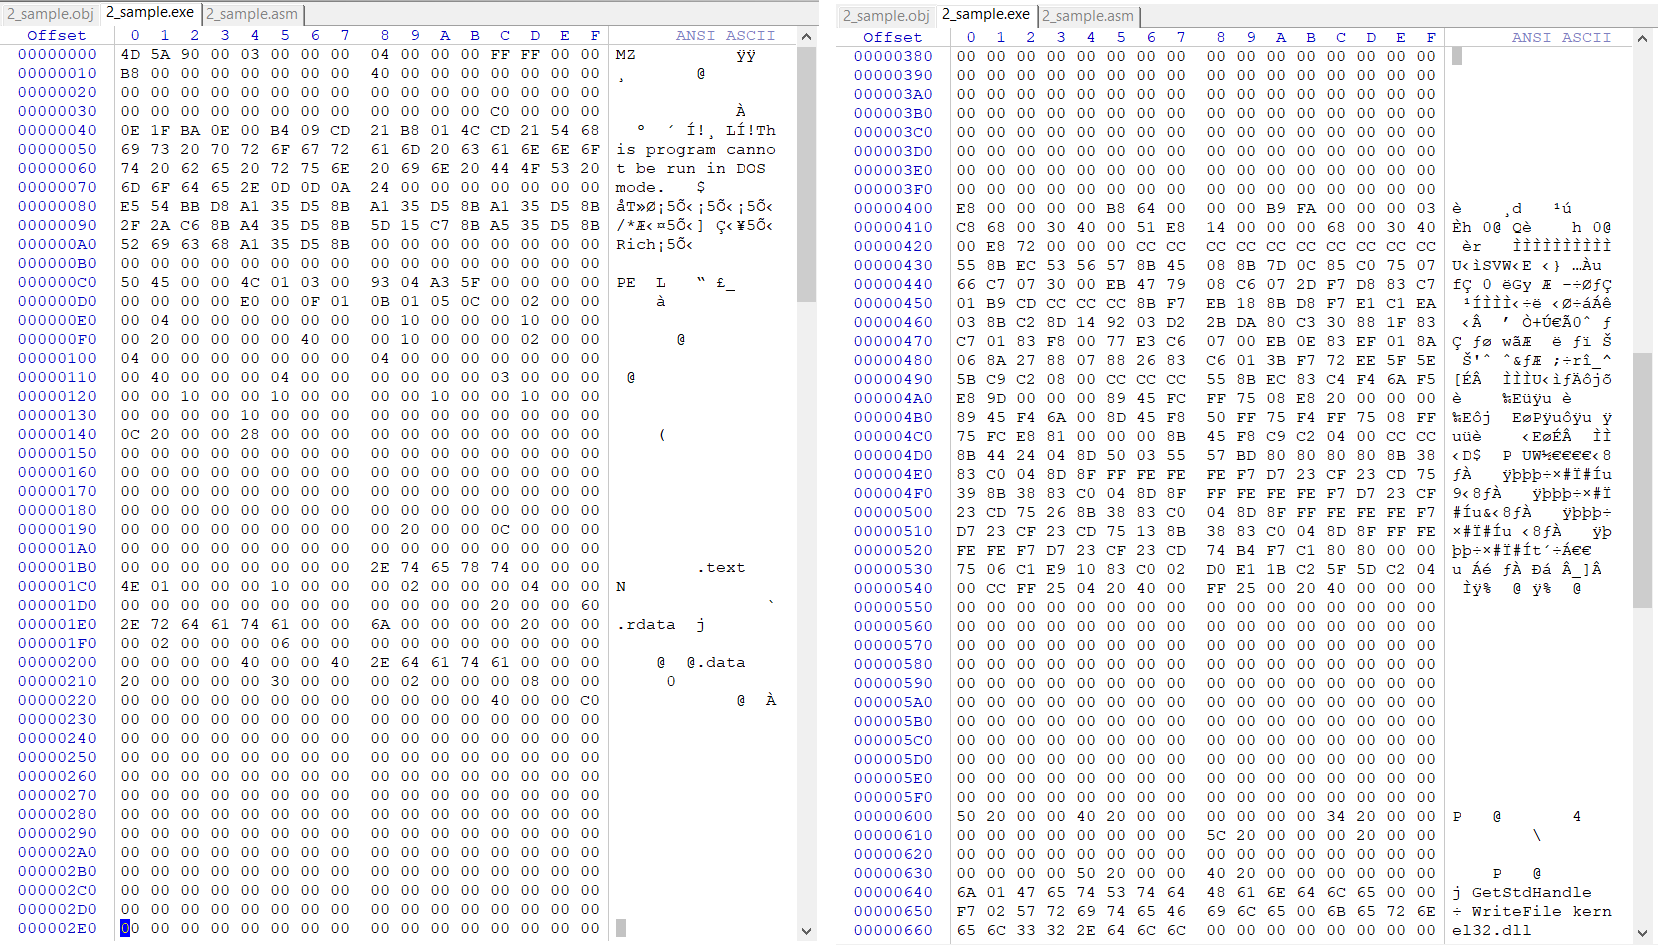
\includegraphics[width=17cm]{WinHexExe.png}
        \caption{Executable Code with WinHex}
        \label{fig:WinHexExe}
\end{figure}

\clearpage
\newpage




\end{document}
